\newlength{\ColumnWidth}
\setlength{\ColumnWidth}{0.315\paperwidth}

\begin{columns}[t]
    \begin{columns}[t,totalwidth=1.0\paperwidth] % split up that three-column-wide column
      \begin{column}{0.25\paperwidth} \begin{MyArticle}[enhanced, tikz={rotate=0}, boxrule=1pt,
  titlerule=0pt, width=0.33\textwidth]{CDF publishes multi-muons!}
  \begin{multicols}{2}
    We report a study of multi-muon events produced at the
    Fermilab Tevatron collider and recorded by the CDF~II detector. In a data 
    set acquired with a dedicated dimuon trigger and corresponding to an 
    integrated luminosity of 2100 pb$^{-1}$, we isolate a significant sample of 
    events in which at least one of the muon candidates is produced 
    outside of the beam pipe of radius 1.5 cm. The production cross section
    and kinematics of events in which both muon candidates are produced inside
    the beam pipe are successfully modeled by known QCD processes which
    include heavy flavor production. In contrast, we are presently unable to 
    fully account for the number and properties of the remaining events, in which
    at least one muon candidate is produced outside of the beam pipe, in terms
    of the same understanding of the CDF~II detector, trigger, and event 
    reconstruction. Several topological and kinematic properties of these 
    events are presented in this paper. These events offer a plausible 
    resolution to long-standing inconsistencies related to $b\bar{b}$
    production and decay.
    \begin{comment}
    % ========================
    \begin{figure}
      \begin{center}
        \vspace{-0.2in}
        \leavevmode
        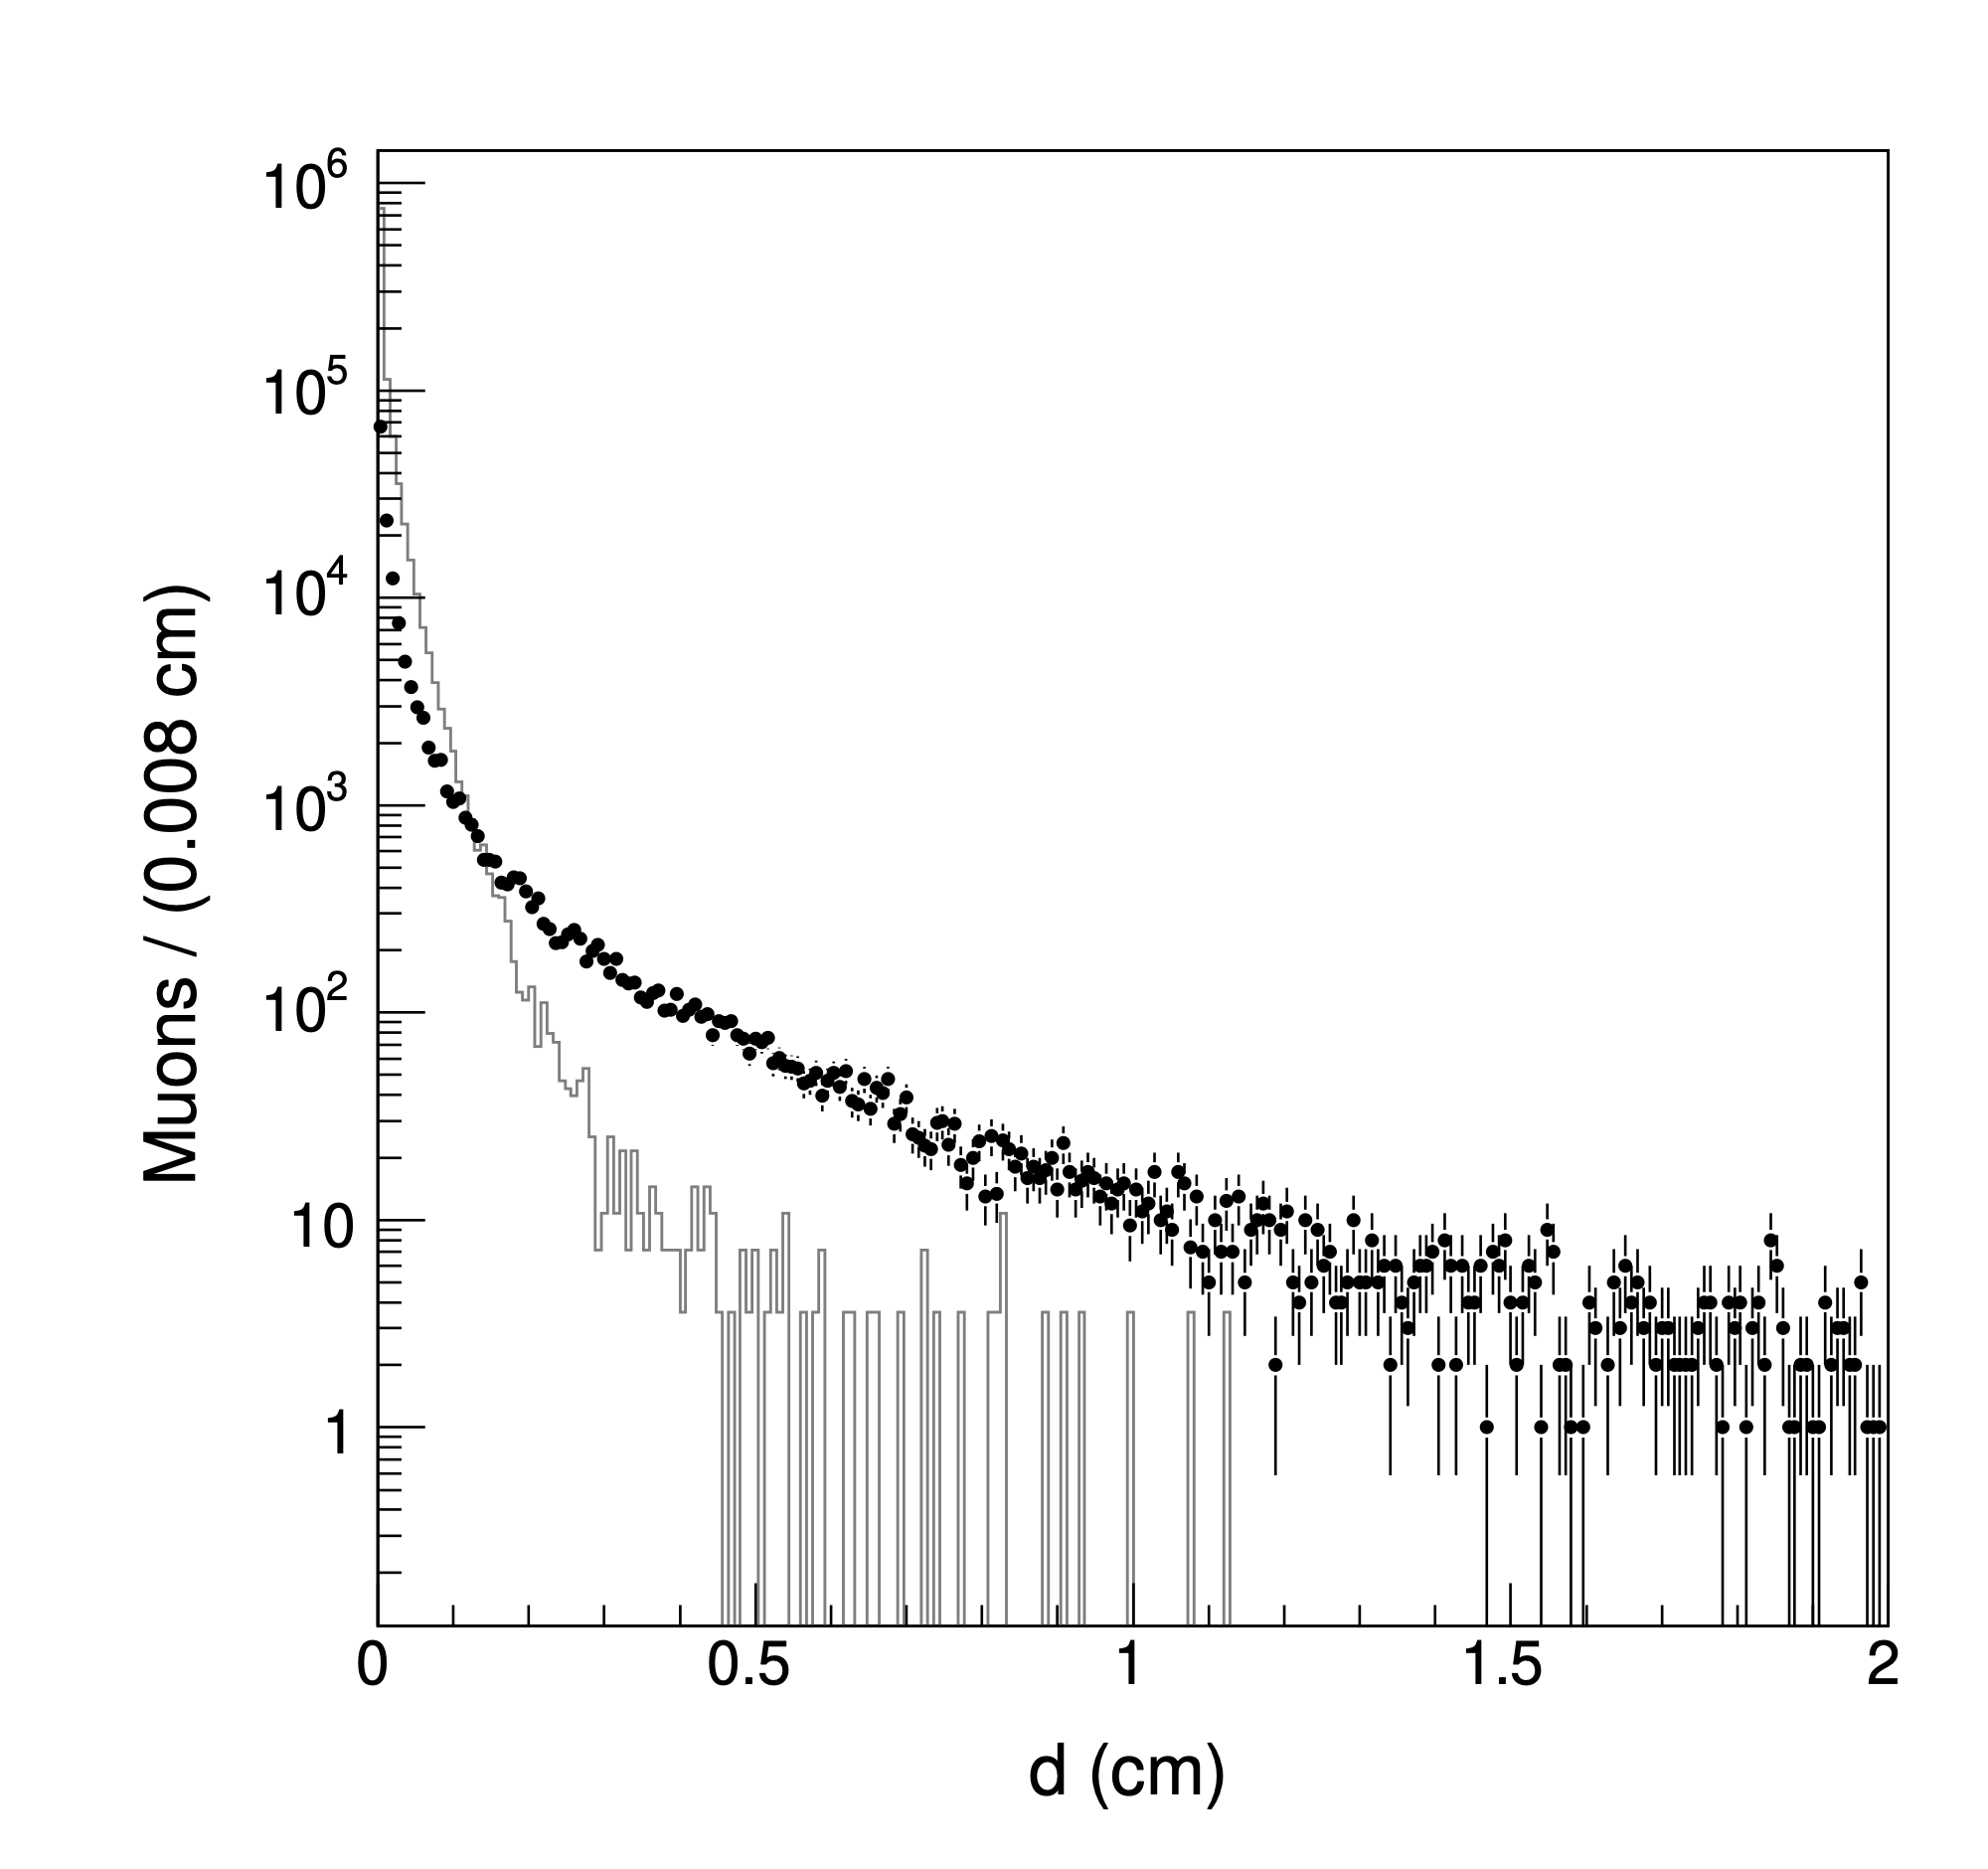
\includegraphics[width=\textwidth]{./figures/MultiMuons1BW_CDF.png}
        %\caption[] {Impact parameter distribution of muons contributed by ghost
        %  ($\bullet$) and QCD (histogram) events. Muon tracks are
        %  selected with loose SVX requirements. The detector resolution
        %  is $\simeq 30 \; \mu$m, whereas bins are 80 $\mu$m wide.} 
      \end{center}
    \end{figure}
    % ========================
    \end{comment}
  \end{multicols}
\end{MyArticle}
 \end{column}
      \begin{column}{0.45\paperwidth} % new tcolorbox environment
\newtcolorbox{headline}[2][]{
  coltext      = black,
  colframe     = \MyBlockFrameColorLeft,
  colback      = \MyBlockFillColorLeft,
  colbacktitle = \MyBlockTitleBoxColor,
  coltitle     = black,
  title        = {\Huge{\textbf{#2}}},
  fonttitle    = \bfseries,
  boxrule      = 0.2cm, %frame line width
  %tikz={rotate=#3}, % manipulate the tcolorbox as a whole (in degrees)
  top=+0.0cm, bottom=+0.0cm, left=+0.05cm, right=+0.05cm,
  %enlarge top by   = +1.0cm,  %  equivalent to mdframed 'skipabove'
  %enlarge bottom by= +0.0cm,  %  equivalent to mdframed 'skipbelow'
  %enlarge left by  = +1.5cm,  
  %enlarge right by = +0.0cm, 
  opacityback=1.0, % 1.0 means totally transparent, 0.0 means totally opaque
  arc=0.0cm,        % 0.0cm for non-rounded corners!
  #1,
}

% CMS
\begin{headline}[enhanced, tikz={rotate=0}]{Fotios Ptochos Promoted to Professor!}
  \begin{multicols}{2}
    \lipsum[1]\\ 
    \lipsum[2]\\ 
    %\lipsum[3]\\ 
    % ========================
    \begin{figure}
      \begin{center}
        \vspace{-0.2in}
        \leavevmode
        \includegraphics[width=0.5\textwidth]{./figures/Fotis6.png}
      \end{center}
    \end{figure}
    % ========================
  \end{multicols}
\end{headline}
 \end{column}
      \begin{column}{0.3\paperwidth} \begin{multimuons-2}[enhanced, tikz={rotate=0}]{Multi-Muons In CDF: The Mystery Continues}
  %\begin{multicols}{2}
    We present a phenomenological conjecture of new physics that is suggested
    by the topology and kinematic properties of the multi-muon events recently
    reported by the CDF collaboration. We show that the salient features of 
    the data can be accounted for by postulating the pair production of
    three new states $h_1$, $h_2$, and $h_3$ with masses in the range
    of 15, 7.3, and 3.6 GeV/c$^{2}$, respectively. The heavier states 
    cascade-decay into the lighter ones, whereas the lightest state 
    decays into a $\tau$ pair with a lifetime of the order of 20 ps.
    \begin{comment}
    % ========================
    \begin{figure}
      \begin{center}
        \vspace{-0.2in}
        \leavevmode
        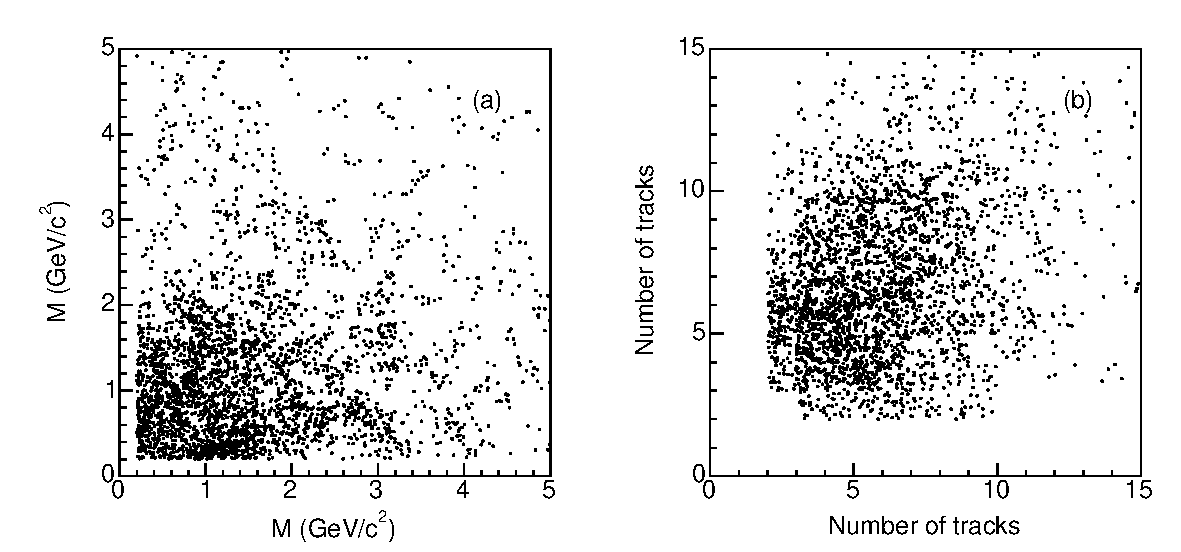
\includegraphics[width=\textwidth]{./figures/MultiMuons2_CDF.pdf}
        %\caption[]{Two-dimensional distributions, reproduced from Ref.~\cite{a0disc},
        %  of (a) the invariant mass, $M$, of all muons and (b) the total
        %  number of tracks contained in a $36.8^{\deg}$ cone when both
        %  cones contain at least two muons.}
      \end{center}
    \end{figure}
    % ========================
    \end{comment}
%  \end{multicols}
\end{multimuons-2}
 \end{column}
    \end{columns}
  \end{columns}

\begin{columns}[t]
    \begin{columns}[t,totalwidth=1.0\paperwidth] % split up that three-column-wide column
      \begin{column}{0.35\paperwidth} \begin{MyArticle}[enhanced, tikz={rotate=0}]{Top Quark, Last Piece of Matter, Appears to Be in Place}
  \begin{multicols}{2}
    We establish the existence of the top quark using a 67 pb$^{-1}$ data
    sample of pp collisions at $\sqrt{s} = 1.8$ TeV collected with the Collider
    Detector at Fermilab (CDF). Employing techniques similar to those we
    previously published, we observe a signal consistent with $t\bar{t}$ decay to
    $WWbb$, but inconsistent with the background prediction by
    4.8$\sigma$. Additional evidence for the top quark is provided by a peak in
    the reconstructed mass distribution. We measure the top quark mass
    to be $176 \pm 8 (\text{stat.}) \pm 10 (\text{sys.})$ GeV/c$^{2}$,
    and the $t\bar{t}$ production cross section to be
    $6.8^{+3.6}_{-2.4}$ pb.
    % ========================
    \begin{figure}
      \begin{center}
        \vspace{-0.2in}
        \leavevmode
        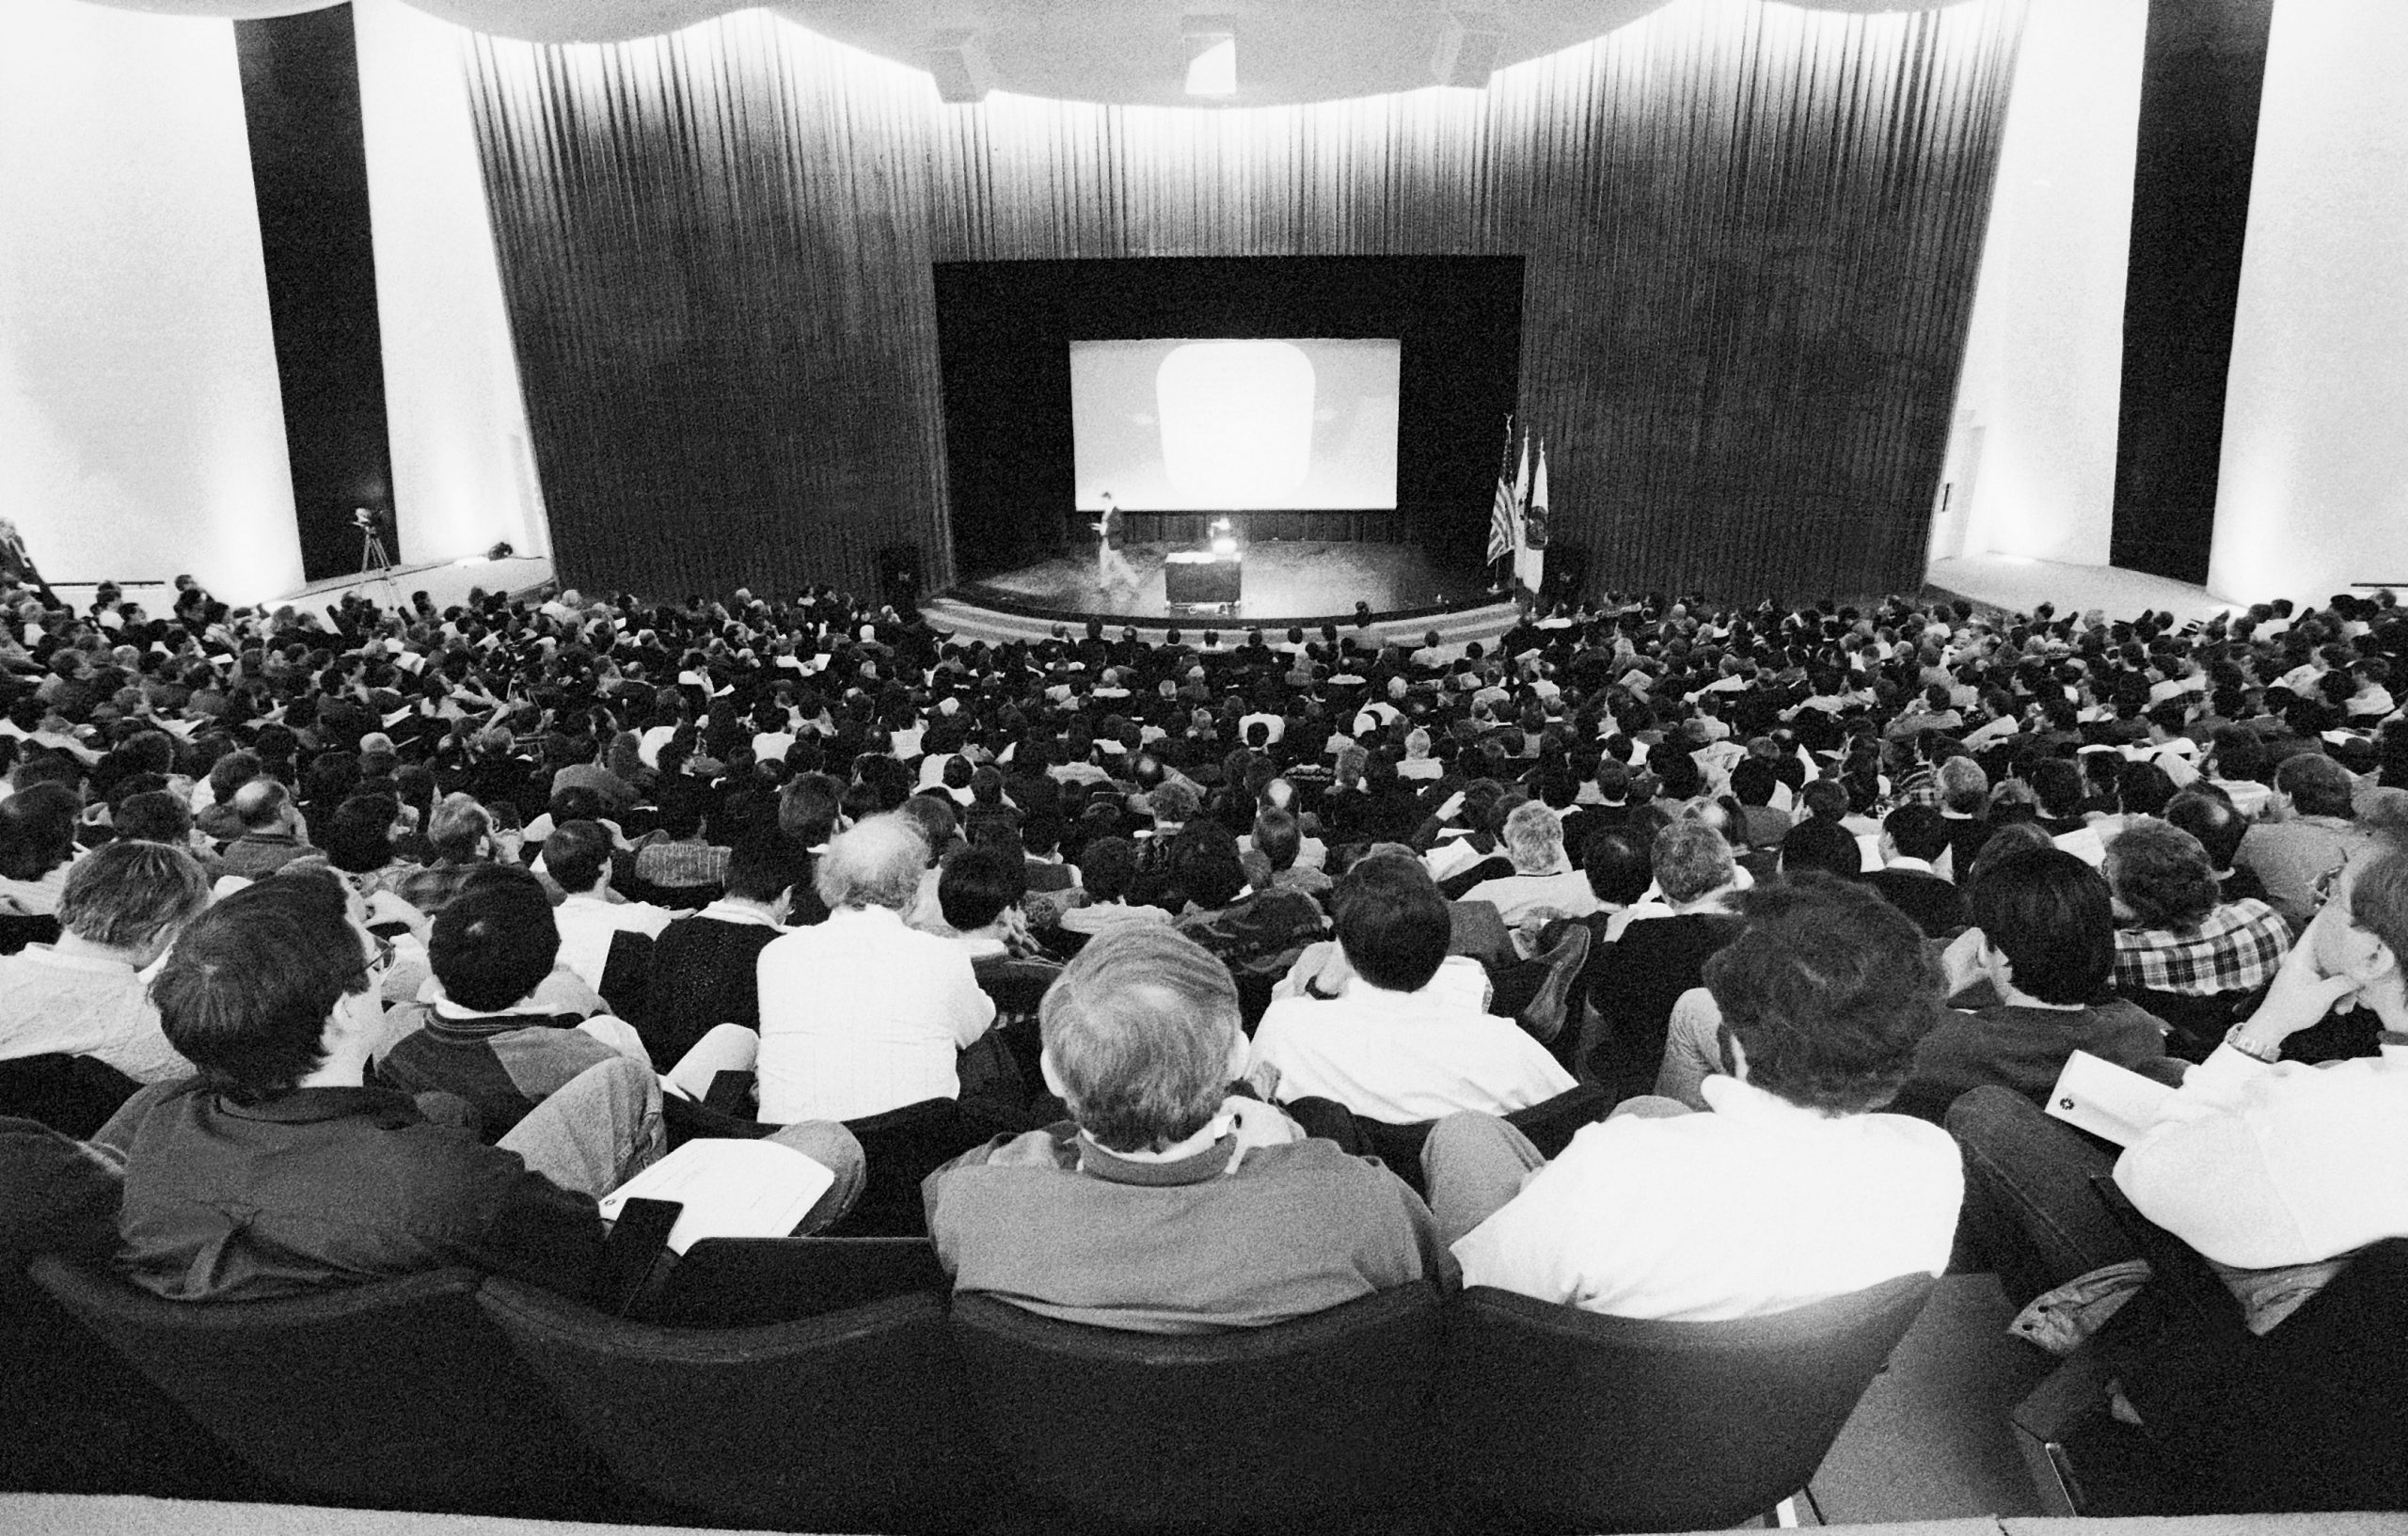
\includegraphics[width=0.5\textwidth]{./figures/TopQuarkAnnouncement.jpg}
      \end{center}
    \end{figure}
    % ========================
  \end{multicols}
\end{MyArticle}
 \end{column}
      \begin{column}{0.35\paperwidth} %\begin{MyArticle}[enhanced, height=0.2\textheight,
%tikz={rotate=0}]{Physicists Find Elusive Particle Seen as Key to
%Universe}
\begin{MyArticle}[enhanced, tikz={rotate=0}, width=0.35\textwidth]{Physicists Find Elusive Particle Seen as Key to Universe}
  \begin{multicols}{2}
    Results are presented from searches for the standard model Higgs
    boson in proton–proton collisions at and 8 TeV in the Compact Muon
    Solenoid experiment at the LHC, using data samples corresponding
    to integrated luminosities of up to 5.1 fb$^{−1}$ at 7 TeV and 5.3 fb$^{−1}$
    at 8 TeV. The search is performed in five decay modes:
    $\gamma\gamma$, $ZZ$,  $\tau^{+}\tau^{-}$, and $b\bar{b}$.
    An excess of events is observed above the expected background,
    with a local significance of 5.0 standard deviations, at a mass
    near 125 GeV, signalling the production of a new particle. The
    expected significance for a standard model Higgs boson of that
    mass is 5.8 standard deviations. The excess is most significant in
    the two decay modes with the best mass resolution, $\gamma\gamma$ and $ZZ$; a
    fit to these signals gives a mass of 
    $125.3\pm0.4(\text{stat.})\pm0.5(\text{syst.}$ GeV. The decay to
    two photons indicates that the new particle is a boson with spin 
    different from one. 
    % ========================
    \begin{figure}
      \begin{center}
        \vspace{-0.2in}
        \leavevmode
        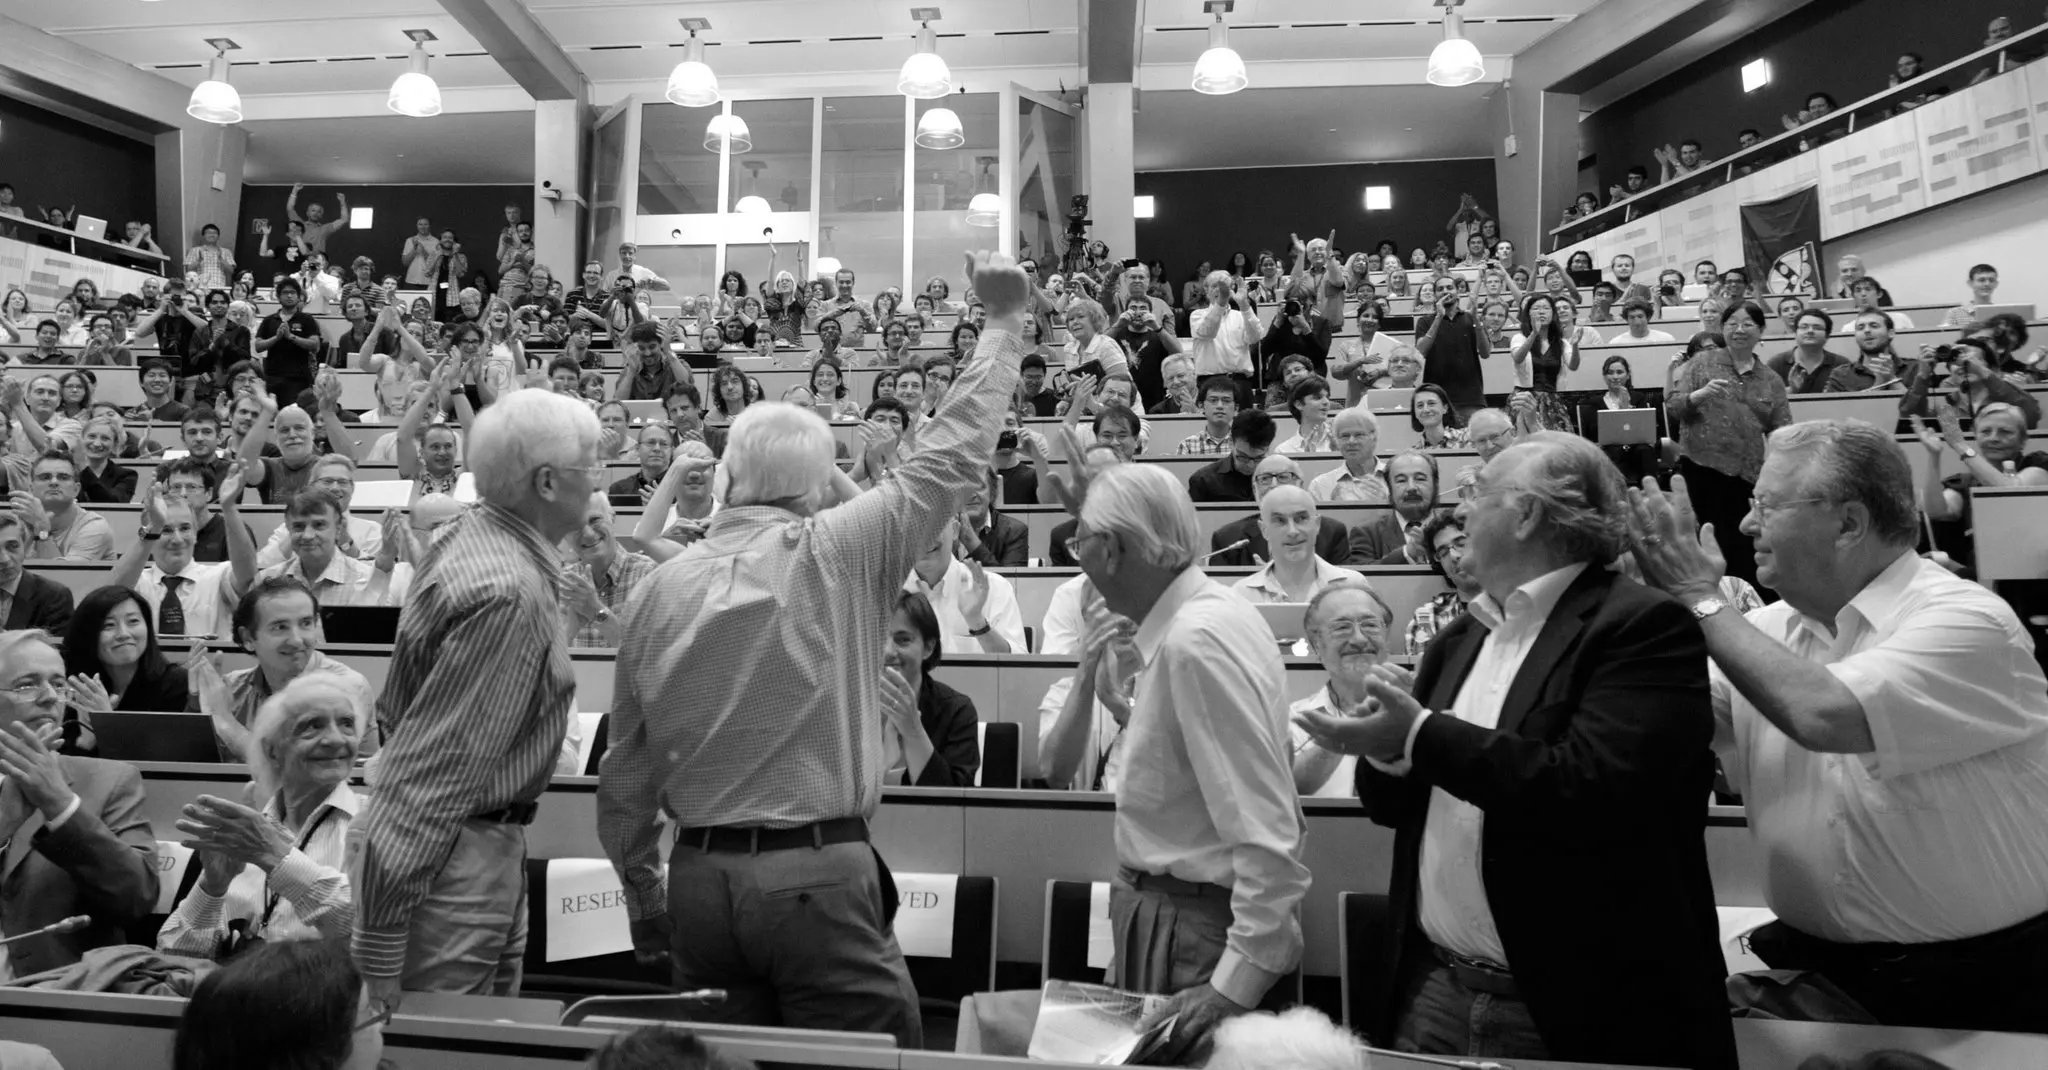
\includegraphics[width=0.5\textwidth]{./figures/HiggsBosonDiscoveryBW.png}
      \end{center}
    \end{figure}
    % ========================
  \end{multicols}
\end{MyArticle}
 \end{column}
    \end{columns}
  \end{columns}
